\documentclass{article}


\usepackage{amsmath} % math stuff
\usepackage{amssymb} % math stuff
\usepackage{array} % equations and stuff
\usepackage{bm} % bold math
%\usepackage{caption} % suppressed table numbering; incompatible with revtex, and longtable, I think
\usepackage{comment} % comment environment
%\usepackage{enumitem} % customization of enumeration, itemize, and description
\usepackage[T1]{fontenc} % font encoding for special characters, must also use scalable font package
\usepackage[margin=0.8in]{geometry} % paper sizes and margins (but be careful not to mess up pre-defined pages)
\usepackage{graphicx} % for graphics
%\usepackage{helvet} % default font is the helvetica postscript font
\usepackage{lipsum} % lorem ipsum filler text
\usepackage{lmodern} % scalable font?
\usepackage{longtable} % multi-page tables
\usepackage{mathrsfs} % math script font
\usepackage{mhchem} % easier chemical formula
\usepackage{microtype} % allows disabling of ligatures
%\usepackage{newcent} % new century schoolbook font
\usepackage{nicefrac}
\usepackage{parskip} % removes paragraph indentation, and adjusts paragraph skip, as well as list items
%\usepackage{setspace} % adjust text spacing and indents
\usepackage{siunitx} % decimal alignment
\usepackage{subfigure} % divided figures
%\usepackage{tabu} % extra table options
\usepackage{textcomp} % symbols
\usepackage{threeparttablex} % better footnotes with longtable
\usepackage{titling} % title placement
\usepackage{ulem} % strikethrough text
%\usepackage{url} % superceded by hyperref
\usepackage{verbatim} % verbatim environment
\usepackage{xcolor} % colors and color boxes
\usepackage{xspace} % commands that don't eat up white space
\usepackage{hyperref} % links and page setup; should always come last

\hypersetup{
	bookmarks=true,
	colorlinks=true,
	citecolor=blue,
	linkcolor=blue,
	urlcolor=blue,
	pdfstartview={XYZ null null 1.0} % default open view is 100%
}

\DisableLigatures[f]{encoding = *, family = * } % disable ff, fi, fl ligatures, without f option, it also disables -- = endash
\renewcommand{\arraystretch}{1.1} % extra vertical space in tables

\begin{document}

\pagestyle{empty} % don't number pages

% custom title
\begin{center}
{\LARGE Classic Riddler}

\vspace{0.15in}

{\Large 21 August 2020}
\end{center}


\section*{Riddle:}

Quarantined in your apartment, you decide to entertain yourself by building a large pen for your pet hamster.
To create the pen, you have several vertical posts, around which you will wrap a sheet of fabric.
The sheet is 1 meter long---meaning the perimeter of your pen can be at most 1 meter---and weighs 1 kilogram, while each post weighs $k$ kilograms.

Over the course of a typical day, your hamster gets bored and likes to change rooms in your apartment.
That means you want your pen to be lightweight and easy to move between rooms.
The total weight of the posts and the fabric you use should not exceed 1 kilogram.

For example, if $k=0.2$, then you could make an equilateral triangle with a perimeter of 0.4 meters (since 0.4 meters of the sheet would weigh 0.4 kilograms), or you could make a square with perimeter of 0.2 meters.
However, you couldn't make a pentagon, since the weight of five posts would already hit the maximum and leave no room for the sheet.

You want to figure out the best shape in order to enclose the largest area possible.
What's the greatest value of $k$ for which you should use four posts rather than three?

\textit{Extra credit}: For which values of $k$ should you use five posts, six posts, seven posts, and so on?

\section*{Solution:}

The approach to this problem is to find the maximum enclosed area for a given number of posts, as a function of $k$.
For $N$ posts, I will call this area function $A_{N}(k)$.
The maximum area for a given $N$ is always a regular $N$-gon using all the available fabric within the weight requirement.
And of course, the concept of area only applies for $N\geq3$.

If each side of the $N$-gon has length $\ell$, then the weight of the posts and the fabric will total one:
\[
N\ell+Nk=1
\]
or
\[
\ell=\frac{1-Nk}{N}
\]

The $N$-gon can be divided up into isosceles triangles, one for each side as shown below:

\vspace{0.1in}
\begin{center}
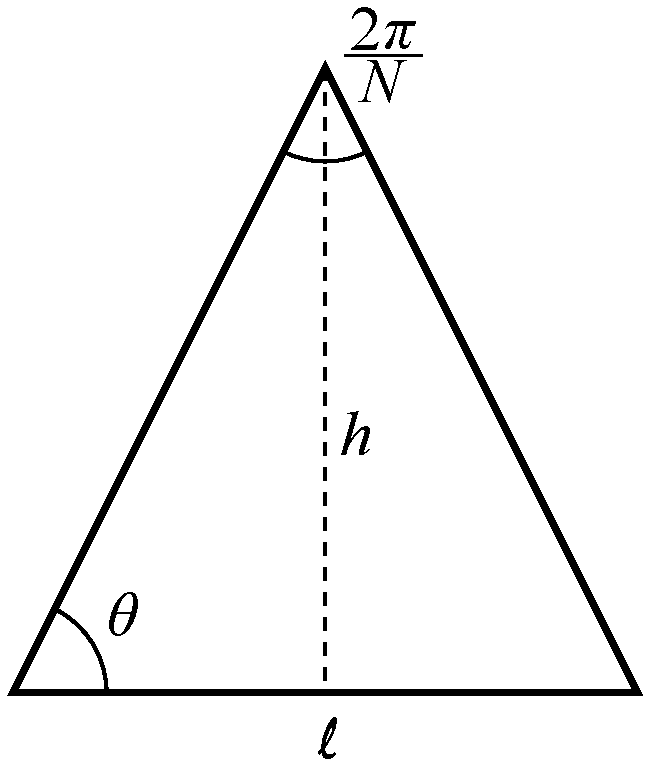
\includegraphics[width=2in]{polygon_section.pdf}
\end{center}
\vspace{0.1in}

Based on the triangle, the angle $\theta$ can be written as 
\[
\theta=\frac{\pi}{2}-\frac{\pi}{N}\ .
\]
The area $A$ of each triangle is of course
\[
A=\frac{1}{2}\ell h\ ,
\]
and the height of the triangle is
\[
h=\frac{\ell}{2}\tan\theta\ .
\]
There are $N$ triangles in the total $N$-gon, and the total area is therefore
\[
A_{N}=\frac{(1-Nk)^{2}}{4N}\tan\left(\frac{\pi}{2}-\frac{\pi}{N}\right)
\]

I expanded these numerically for several $N$:

\vspace{0.1in}
\begin{center}
\begin{tabular}{c c}
$N$ & $A_{N}(k)$ \\
\hline
3 & $0.048112(1-3k)^{2}$ \\
4 & $0.0625(1-4k)^{2}$ \\
5 & $0.068819(1-5k)^{2}$ \\
6 & $0.072169(1-6k)^{2}$ \\
7 & $0.074161(1-7k)^{2}$ \\
8 & $0.075444(1-8k)^{2}$
\end{tabular}
\end{center}
\vspace{0.1in}

Each of these is just a parabola, of course, but they are only physically valid for $k$ values between 0 and $\nicefrac{1}{N}$.
The riddle is asking for the curve with the largest area for a given value of $k$.
So the points of intersection of adjacent curves gives the solution, and a start to the extra credit.
I will call the points of intersection $k_{i-j}$ for the intersection of curves $i$ and $j$.
The solution for $k_{3-4}$ (the original riddle), which I solved with the numerical approximations above, is approximatly
\fcolorbox{red}{white}{\bf 0.08965 kg}\,,
so there should be three posts for any mass between 0.08965~kg and 0.33333~kg.
A few other solutions are

\vspace{0.1in}
\begin{center}
\begin{tabular}{c c}
$i-j$ & $k_{i-j}$ \\
\hline
$4-5$ & 0.03957 \\
$5-6$ & 0.02102 \\
$6-7$ & 0.01251 \\
$7-8$ & 0.00806
\end{tabular}
\end{center}
\vspace{0.1in}



\end{document}